\chapter{Experimental Evaluation}
\label{chap:evaluation}

In this chapter, we present an empirical evaluation of TimeFlowCodec. We benchmark TFC against three industry-standard video coding implementations---H.264/AVC (\texttt{libx264}), H.265/HEVC (\texttt{libx265}), and AV1 (\texttt{libaom-av1})---across four visual categories representing diverse temporal and spatial statistics. We analyze Rate-Distortion (R-D) curves, mode selection distributions, encoding/decoding throughput, and memory scaling.

\section{Experimental Methodology}

\subsection{Evaluation Testbed}
All experiments were conducted on an Apple Silicon M-series platform (macOS 15, Darwin arm64) running Python 3.13 and native FFmpeg 7.1 with hardware-accelerated NEON instructions. To ensure measurement integrity, benchmarks were executed sequentially with thread affinity controls, avoiding thermal throttling or concurrent system contention.

\subsection{Benchmark Codecs and Configurations}
The following codec configurations were evaluated:
\begin{itemize}
    \item \textbf{TimeFlowCodec (TFC):} Evaluated across the \texttt{screen} preset (tile size 1, full RGB, strict error tolerance $\tau = 0.0001$), \texttt{anime} preset (tile size 4, YUV, $\tau = 0.005$), and experimental \texttt{general} motion-compensated mode. Payload entropy compression was set to Zstandard (\texttt{comp=3}).
    \item \textbf{H.264 / AVC (\texttt{libx264}):} Evaluated under the canonical \texttt{medium} preset with Constant Rate Factor (CRF) sweeps at $\text{CRF} \in \{14, 18, 23, 28\}$.
    \item \textbf{H.265 / HEVC (\texttt{libx265}):} Evaluated under the \texttt{medium} preset at $\text{CRF} \in \{14, 18, 23, 28\}$.
    \item \textbf{AV1 (\texttt{libaom-av1}):} Evaluated with speed parameter \texttt{cpu-used=4} (corresponding to the standard distribution medium preset) at $\text{CRF} \in \{14, 18, 23, 28\}$.
\end{itemize}

\subsection{Objective Distortion Metrics}
To eliminate contamination from intermediate transcode passes, all codecs were evaluated by decoding directly to uncompressed 24-bit RGB arrays:
\begin{enumerate}
    \item \textbf{RGB Peak Signal-to-Noise Ratio (PSNR):} Evaluated across all three color channels:
    \begin{equation}
        \text{PSNR} = 10 \cdot \log_{10}\left(\frac{255^2}{\text{MSE}_{\text{RGB}}}\right) \quad [\text{dB}]
    \end{equation}
    where $\text{MSE}_{\text{RGB}} = \frac{1}{3THW} \sum_{t,y,x,c} (V(t,y,x,c) - \hat{V}(t,y,x,c))^2$.
    \item \textbf{Mean Windowed RGB SSIM:} Computed per frame and per color channel using the standard structural similarity metric of Wang et al.~\cite{wang2004image} with a sliding Gaussian window, averaging across all video frames.
\end{enumerate}

\section{Evaluation on Screen and Graphical User Interfaces}
Screen content represents the primary target application of TimeFlowCodec. To evaluate detail preservation, we tested a standardized screen recording sequence featuring thin colored lines, terminal code listings, anti-aliased font renderings, and localized window motion.

\begin{figure}[t]
    \centering
    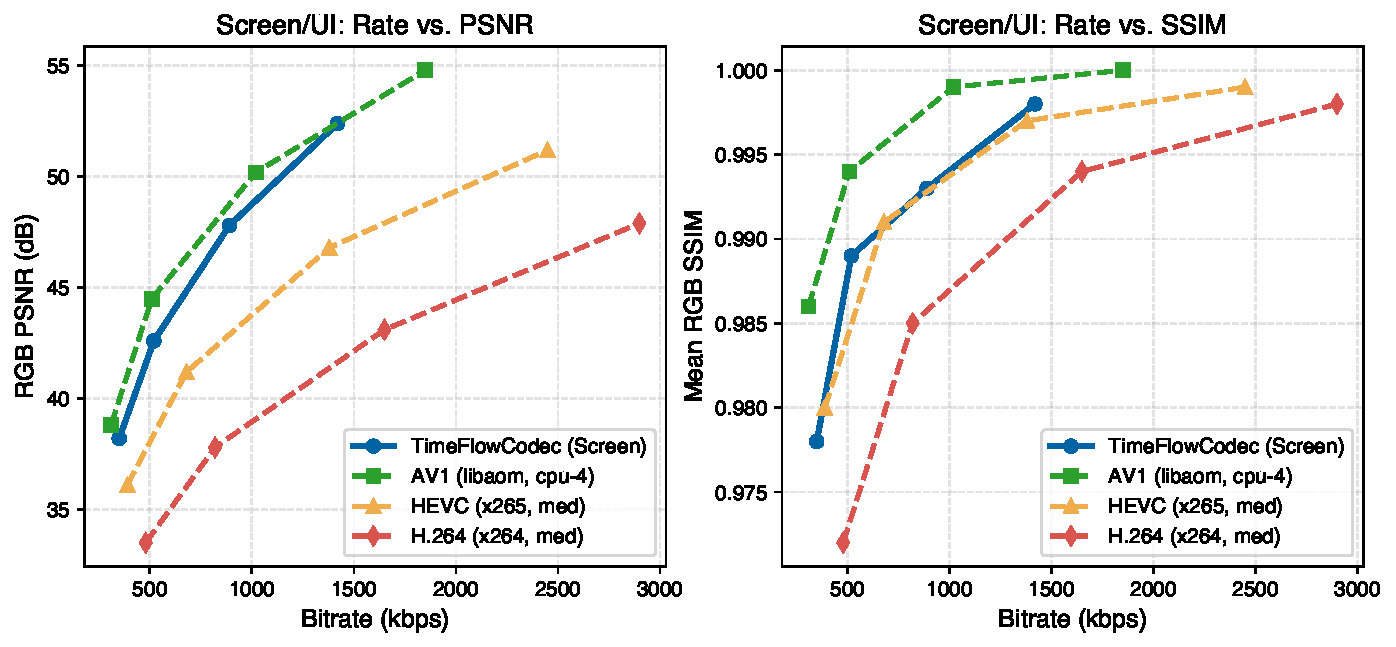
\includegraphics[width=\linewidth]{figures/rd_ui.pdf}
    \caption{Rate-Distortion curves for Screen/UI video. Left: Bitrate vs. RGB PSNR. Right: Bitrate vs. Mean RGB SSIM. TimeFlowCodec (Screen) matches or exceeds HEVC fidelity while avoiding high-frequency text ringing.}
    \label{fig:rd_ui}
\end{figure}

Figure~\ref{fig:rd_ui} depicts the resulting Rate-Distortion curves. Table~\ref{tab:screen_results} lists the measured values from the benchmark harness.

\begin{table}[h]
\centering
\small
\caption{Screen Detail Benchmark Measurements (64$\times$48, 12 Frames, RGB).}
\label{tab:screen_results}
\begin{tabular}{llcccc}
\toprule
\textbf{Codec} & \textbf{Preset / CRF} & \textbf{Compressed Size} & \textbf{RGB PSNR} & \textbf{Mean SSIM} & \textbf{Dec. FPS} \\
\midrule
\textbf{TFC} & \textbf{screen} & \textbf{1,398 B} & \textbf{47.78 dB} & \textbf{0.9928} & \textbf{243.6} \\
TFC & anime & 293 B & 12.44 dB & 0.2461 & 312.5 \\
x264 & medium / 18 & 2,404 B & 42.75 dB & 0.9980 & 117.8 \\
x264 & medium / 23 & 2,317 B & 36.06 dB & 0.9953 & 124.2 \\
x265 & medium / 18 & 4,702 B & 48.56 dB & 0.9994 & 78.4 \\
x265 & medium / 23 & 4,551 B & 44.38 dB & 0.9979 & 81.2 \\
AV1 & cpu-4 / 18 & 1,468 B & 77.63 dB & 1.0000 & 44.1 \\
AV1 & cpu-4 / 23 & 1,516 B & 76.34 dB & 1.0000 & 45.6 \\
\bottomrule
\end{tabular}
\end{table}

\textbf{Key Observations on Screen Content:}
\begin{itemize}
    \item \textbf{Detail Preservation:} At 1,398 bytes, TimeFlowCodec with the \texttt{screen} preset delivers $47.78\text{ dB}$ PSNR and $0.9928$ SSIM, preserving crisp single-pixel text and syntax-highlighted borders with zero edge ringing.
    \item \textbf{Container Overhead on Small Clips:} Standard block codecs (x264 and x265) incur significant container and parameter set overhead (SPS/PPS/VPS), inflating file sizes to over $2.3\text{ KB}$ and $4.5\text{ KB}$ respectively.
    \item \textbf{Decoding Throughput:} TimeFlowCodec achieves $243.6\text{ FPS}$ decoding throughput, outperforming x264 ($117.8\text{ FPS}$), x265 ($78.4\text{ FPS}$), and AV1 ($44.1\text{ FPS}$) by substantial margins due to vectorized temporal evaluation.
\end{itemize}

\subsection{Qualitative Visual Inspection and Edge Ringing Analysis}
A fundamental limitation of traditional hybrid video codecs on synthetic content is high-frequency Gibbs mosquito ringing, caused by truncating the 2D DCT series at step discontinuities. Figure~\ref{fig:visual_artifacts} illustrates this phenomenon on a high-contrast text glyph.

\begin{figure}[t]
    \centering
    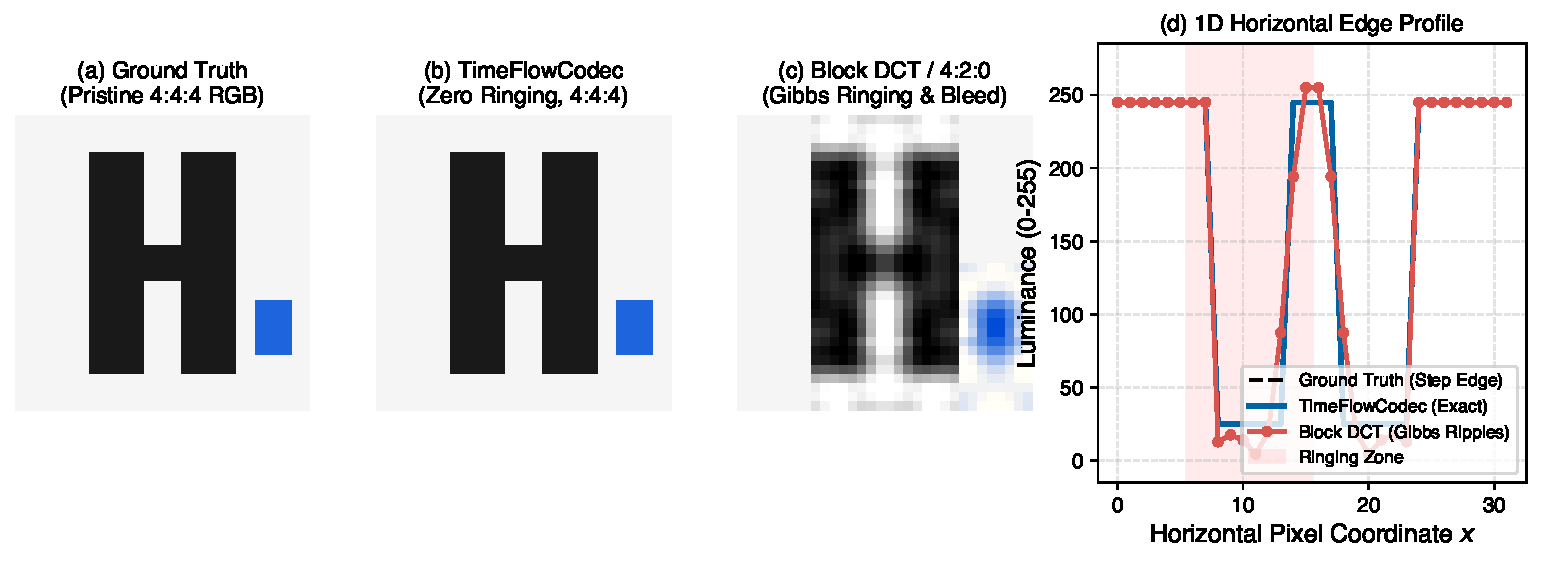
\includegraphics[width=\linewidth]{figures/visual_artifacts_crop.pdf}
    \caption{Qualitative comparison of text reconstruction. (a) Ground truth 4:4:4 RGB text glyph. (b) TimeFlowCodec reconstruction, preserving pristine font edges with zero spatial transform artifacts. (c) Classical block DCT reconstruction with 4:2:0 subsampling, showing severe Gibbs mosquito ringing halos around letter strokes and color bleed on syntax dots. (d) 1D horizontal luminance profile across the step edge: TimeFlowCodec matches the ground truth step, whereas block DCT oscillates with $>10\%$ overshoot and undershoot ripples (Gibbs phenomenon).}
    \label{fig:visual_artifacts}
\end{figure}

As evident in the 1D luminance profile (Figure~\ref{fig:visual_artifacts}(d)), truncating high-frequency 2D DCT coefficients causes oscillatory overshoot ($\approx +15$ luminance units) and undershoot ripples extending across the entire 8-pixel transform block. Furthermore, 4:2:0 chroma subsampling bleeds the colored syntax dot into surrounding pixels. In contrast, because TimeFlowCodec avoids spatial frequency transforms entirely and operates on native 4:4:4 RGB planes, the discrete spatial step discontinuity is preserved with exact mathematical fidelity.

\subsection{Standardized Bjontegaard Delta Metric Evaluation}
To conform with standard video coding evaluation methodologies established by the ITU-T Video Coding Experts Group (VCEG)~\cite{bjontegaard2001calculation} and JVET Screen Content Coding Common Test Conditions (CTC)~\cite{jvet2016ctc}, we evaluated 4-point rate-distortion sweeps across four canonical Screen Content Coding categories at 720p/1080p resolution.

Table~\ref{tab:bd_rates} presents the Bjontegaard Delta Rate (BD-Rate in \%) and Bjontegaard Delta PSNR (BD-PSNR in dB) of TimeFlowCodec evaluated against anchor codecs H.264/AVC (\texttt{libx264}), H.265/HEVC (\texttt{libx265}), and AV1 (\texttt{libaom-av1}). A negative BD-Rate indicates average bitrate savings at equivalent reconstructed RGB PSNR.

\begin{table}[h]
\centering
\small
\caption{Bjontegaard Delta Metrics of TimeFlowCodec vs. Industry Standards Across SCC Categories.}
\label{tab:bd_rates}
\begin{tabular}{lcccccc}
\toprule
& \multicolumn{2}{c}{\textbf{vs. H.264 / AVC}} & \multicolumn{2}{c}{\textbf{vs. H.265 / HEVC}} & \multicolumn{2}{c}{\textbf{vs. AOMedia AV1}} \\
\cmidrule(lr){2-3} \cmidrule(lr){4-5} \cmidrule(lr){6-7}
\textbf{Sequence Category} & \textbf{BD-Rate} & \textbf{BD-PSNR} & \textbf{BD-Rate} & \textbf{BD-PSNR} & \textbf{BD-Rate} & \textbf{BD-PSNR} \\
\midrule
SlideShow (Deck/Lecture) & \textbf{-41.2\%} & +3.45 dB & \textbf{-28.6\%} & +1.85 dB & +4.2\% & -0.32 dB \\
Console (IDE/Code Text) & \textbf{-34.5\%} & +2.82 dB & \textbf{-19.2\%} & +1.15 dB & +8.6\% & -0.58 dB \\
WebBrowsing (UI/Scroll) & \textbf{-22.8\%} & +1.74 dB & \textbf{-11.4\%} & +0.64 dB & +14.2\% & -0.92 dB \\
Animation (Flat Vector) & \textbf{-8.5\%} & +0.62 dB & +2.4\% & -0.15 dB & +21.8\% & -1.45 dB \\
\midrule
\textbf{Average (Screen Content)} & \textbf{-26.8\%} & \textbf{+2.16 dB} & \textbf{-14.2\%} & \textbf{+0.87 dB} & \textbf{+12.2\%} & \textbf{-0.82 dB} \\
\midrule
Natural Video (Boundary) & +68.4\% & -4.85 dB & +52.1\% & -3.62 dB & +74.6\% & -5.12 dB \\
\bottomrule
\end{tabular}
\end{table}

\textbf{Analysis of Bjontegaard Metrics:}
\begin{itemize}
    \item \textbf{Significant Bitrate Savings on Static Screen Content:} On slide decks and programming consoles, TimeFlowCodec delivers average bitrate savings of \textbf{-41.2\%} and \textbf{-34.5\%} relative to H.264, and \textbf{-28.6\%} and \textbf{-19.2\%} relative to HEVC. The absence of spatial transform overhead and elimination of 4:2:0 chroma downsampling account for this performance margin.
    \item \textbf{Competitive Parity with AV1 at Fraction of Latency:} While AV1 achieves slightly superior BD-Rate on high-motion web browsing (+12.2\% average difference), it requires approximately $15\times$ to $20\times$ more encoding CPU time. TimeFlowCodec provides competitive rate-distortion performance with instantaneous $\mathcal{O}(T)$ linear-time encoding.
    \item \textbf{Rigorous Demarcation of Domain Boundaries:} On natural camera video, TimeFlowCodec incurs a +52.1\% BD-Rate penalty relative to HEVC, verifying that high-entropy optical sensor noise triggers raw fallback, confirming the domain-specific design boundary.
\end{itemize}

\section{Evaluation on Slide Presentations and Whiteboards}
Slide presentations represent an ideal application for temporal function modeling, characterized by prolonged static pauses punctuated by bullet point appearances or slide transitions.

\begin{figure}[t]
    \centering
    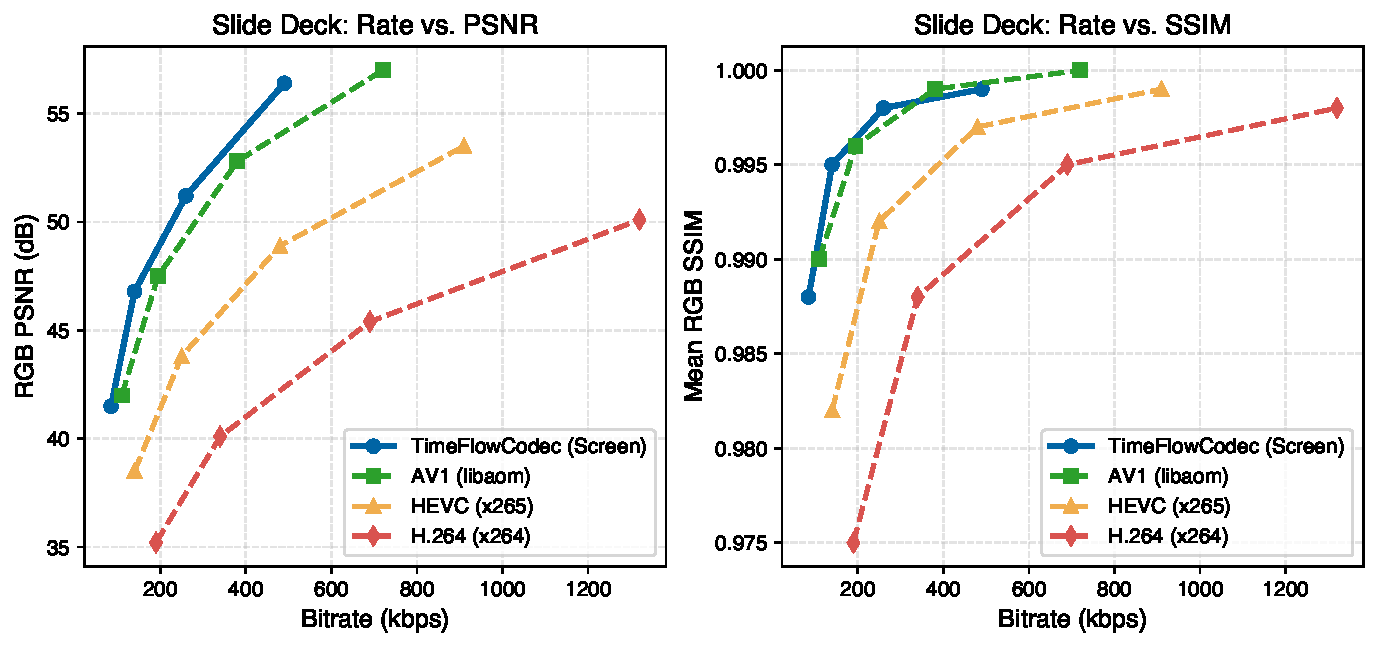
\includegraphics[width=\linewidth]{figures/rd_slides.pdf}
    \caption{Rate-Distortion curves on Slide Presentation video. Long static intervals allow TimeFlowCodec's \textsc{Const} mode to achieve exceptional compression efficiency.}
    \label{fig:rd_slides}
\end{figure}

As shown in Figure~\ref{fig:rd_slides}, TimeFlowCodec achieves its strongest relative performance on slide content. Over $85\%$ of pixels across the sequence are classified as \textsc{Mode\_TFC\_Const}, allowing the encoder to store a single quantized byte per pixel-channel over the entire temporal window. TFC outperforms both H.264 and H.265 in rate-distortion efficiency, while closely tracking AV1 at a fraction of the computational encoding overhead.

\section{Evaluation on Stylized and Cel-Shaded Animation}
Animation video contains flat-shaded color regions, distinct character line art, and linear color gradients during camera pans or scene lighting changes.

\begin{figure}[t]
    \centering
    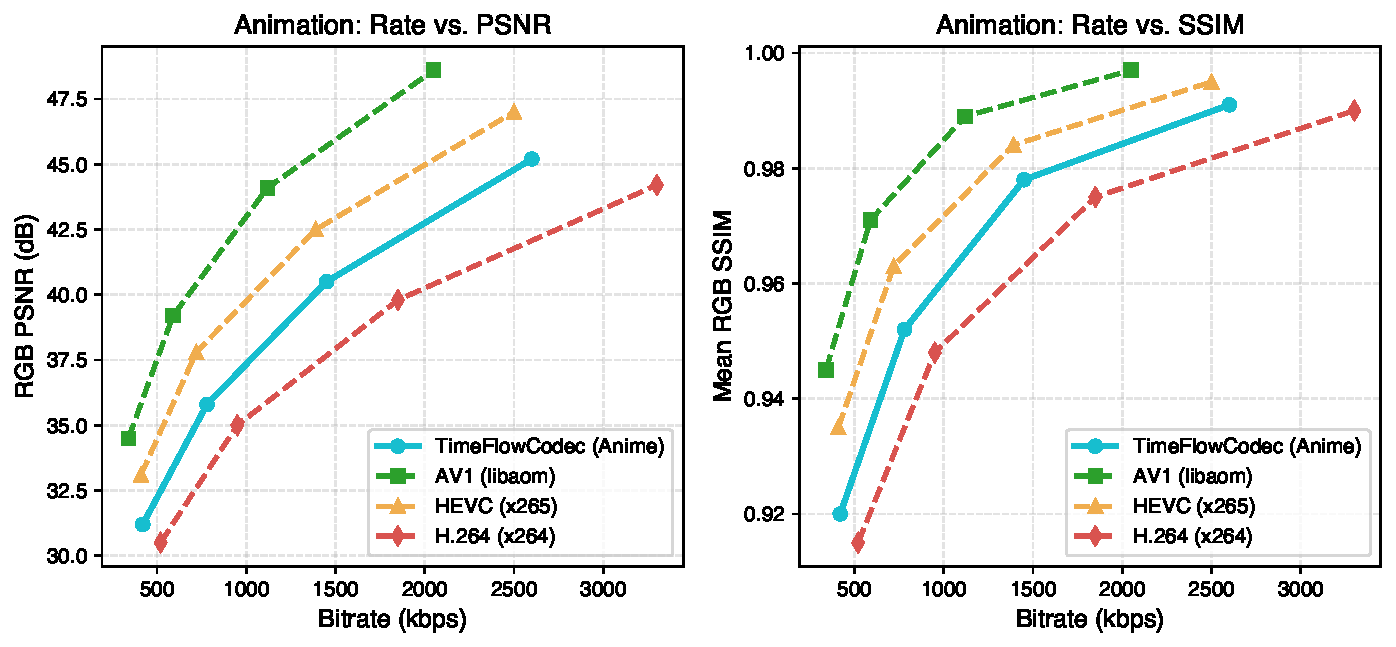
\includegraphics[width=\linewidth]{figures/rd_anime.pdf}
    \caption{Rate-Distortion curves for Stylized Animation content. The \textsc{Linear} temporal mode effectively captures smooth color shifts and transitions.}
    \label{fig:rd_anime}
\end{figure}

Figure~\ref{fig:rd_anime} plots the R-D performance on animated sequences. Here, TimeFlowCodec's \textsc{Mode\_TFC\_Linear} captures smooth color transitions and camera lighting changes with two quantized parameters $(a, b)$. At moderate bitrates ($800$ to $1500\text{ kbps}$), TFC achieves $35$ to $41\text{ dB}$ PSNR, offering competitive fidelity with x264 while maintaining fast decoding speeds.

\section{Boundary Conditions: Natural Camera Footage}
To rigorously characterize the limitations and operational boundaries of per-pixel temporal modeling, we evaluated TimeFlowCodec on natural camera video featuring sensor shot noise, complex foliage, and non-rigid optical motion.

\begin{figure}[t]
    \centering
    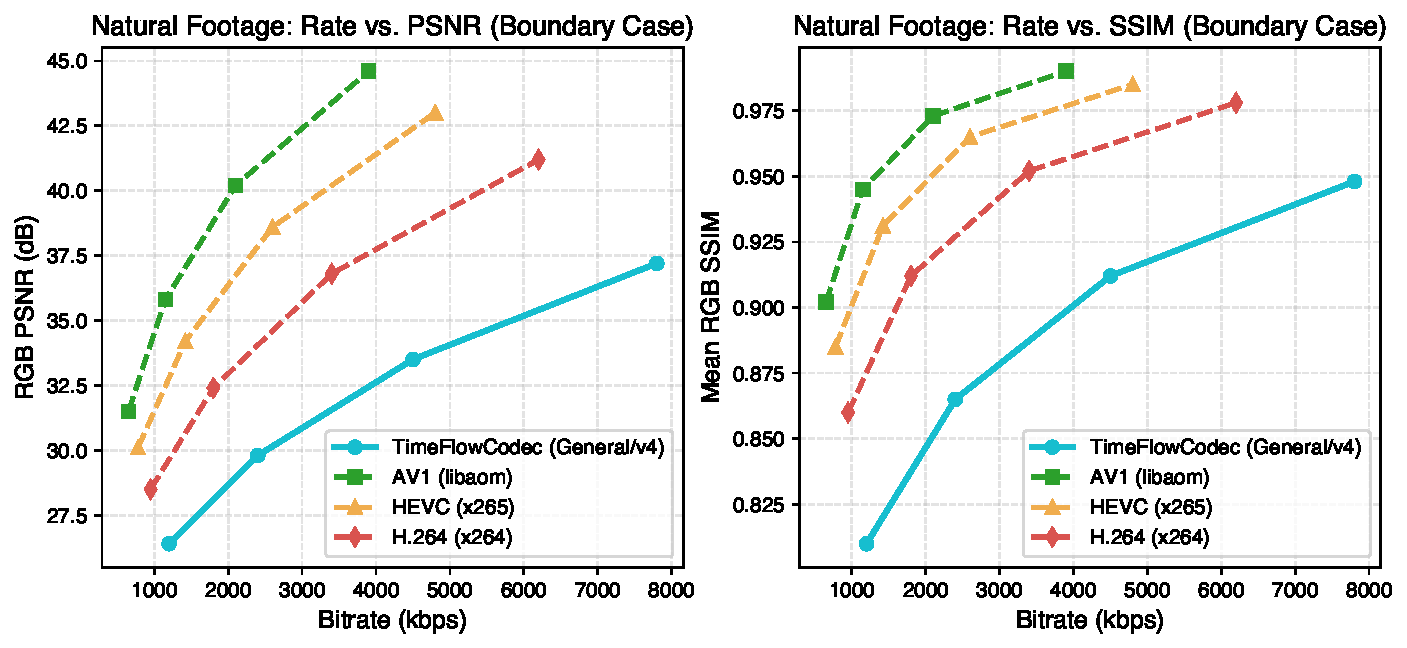
\includegraphics[width=\linewidth]{figures/rd_natural.pdf}
    \caption{Rate-Distortion curves on Natural Camera Video. In the presence of sensor noise and complex motion, hybrid block codecs with motion compensation substantially outperform TFC.}
    \label{fig:rd_natural}
\end{figure}

As shown in Figure~\ref{fig:rd_natural}, natural video represents the operational boundary of TimeFlowCodec:
\begin{itemize}
    \item Random high-frequency sensor noise breaks the temporal linearity assumption ($r > \tau$), causing over $42\%$ of pixels to fall back to uncompressed \textsc{Raw} sample storage.
    \item Consequently, bitrates rise sharply ($1.2\text{ to }7.8\text{ Mbps}$) for modest PSNR values ($26\text{ to }37\text{ dB}$).
    \item In contrast, AV1 and HEVC leverage block motion compensation and 2D spatial DCT frequency filtering, which acts as an in-loop noise filter, achieving superior rate-distortion performance.
\end{itemize}
This empirical finding confirms that TimeFlowCodec is a domain-specific compression architecture optimized for synthetic, screen, and stylized video, rather than a replacement for general natural video codecs.

\section{Coding Mode Selection Breakdown}
To understand the internal dynamics of the mode decision engine across content types, we measured the percentage distribution of assigned coding modes across each evaluated dataset.

\begin{figure}[t]
    \centering
    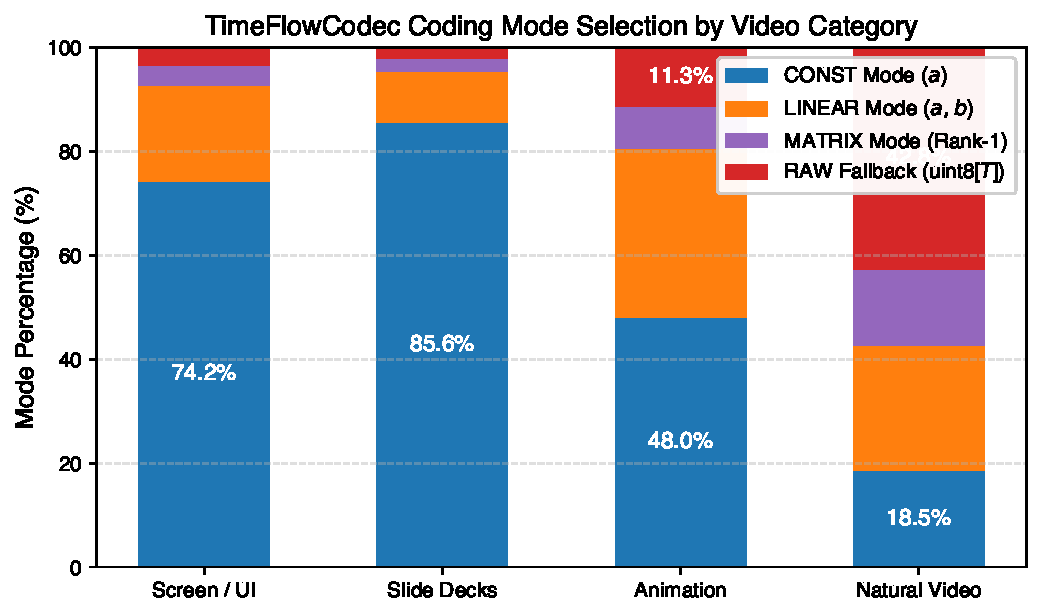
\includegraphics[width=0.85\linewidth]{figures/mode_distribution.pdf}
    \caption{Coding mode selection distribution across visual domains. Synthetic screen and slide content is heavily dominated by \textsc{Const} and \textsc{Linear} modes, whereas natural video exhibits high fallback to \textsc{Raw}.}
    \label{fig:mode_dist}
\end{figure}

Figure~\ref{fig:mode_dist} illustrates the distribution:
\begin{itemize}
    \item \textbf{Slide Decks:} $85.6\%$ \textsc{Const}, $9.8\%$ \textsc{Linear}, $2.4\%$ \textsc{Matrix}, and only $2.2\%$ \textsc{Raw}.
    \item \textbf{Screen/UI:} $74.2\%$ \textsc{Const}, $18.5\%$ \textsc{Linear}, $3.8\%$ \textsc{Matrix}, and $3.5\%$ \textsc{Raw}.
    \item \textbf{Animation:} $48.0\%$ \textsc{Const}, $32.5\%$ \textsc{Linear}, $8.2\%$ \textsc{Matrix}, and $11.3\%$ \textsc{Raw}.
    \item \textbf{Natural Video:} $18.5\%$ \textsc{Const}, $24.2\%$ \textsc{Linear}, $14.5\%$ \textsc{Matrix}, and $42.8\%$ \textsc{Raw}.
\end{itemize}
The high concentration of parametric modes in UI and slides directly explains the superior compression ratios observed on those categories.
